\documentclass[11pt]{article}
\usepackage{fullpage}
\usepackage{graphicx}
\usepackage{natbib}

\begin{document}
\title{Radio Skillz: Analog Lab 1}

\maketitle

\section*{Prerequisites}

Reading: Horowitz \& Hill, Ch. 1

\begin{itemize}
\item Ohm's Law
\item Th\'evenin Equivalent Resistance
\item Capacitance and Inductance
\item RC Filters
\item Diodes
\end{itemize}

\section*{Materials}

\begin{itemize}
\item breadboard
\item misc R, C, L components
\item potentiometer (``pot'')
\item power supply
\item function generator w/ external FM reference
\item oscilloscope w/ probes
\item voltimeter
\item speaker w/ amplifier
\end{itemize}

\section*{Some Thoughts}

\subsection*{Breadboards}

Breadboards are convenient for constructing circuts for this lab.  Take some time to get to know yours
using a ohmmeter.  In particular, figure out what is connected, and what is not.

\subsection*{Grounding}

Ground means different things in different contexts (e.g. earth ground, signal ground,
chassis ground).  For our purposes in
this lab, ground simply provides a return path for current.  We define it to be
0V (i.e. it is the reference from which we measure voltage differences).  The
ground of your circuit should be tied to the ground of your power supply.  It
is good practice to consistently use a color (black, blue, and green are good
choices) to indicate ground lines in your circuits.

\subsection*{Capacitor Orientation}

Some capacitors, particularly electrolytics, care about which direction voltage
is applied across them.  Often, one of the leads is longer, and may have a `+'
near it on the body of the capacitor.  Always connect this lead to the higher voltage.
Failure to do so can, for higher voltages, cause them to explode.

\subsection*{Oscilloscopes}

'Scopes can be intimidating.  The solution is to press buttons until they submit.  Seriously, don't be afraid
to push buttons.  In order to show a static display of a repeating signal, scopes need to trigger on
some edge of an input signal.  This is always configurable, and you'll need to figure out how.  You can
adjust the time (X axis) and voltage (Y axis) ranges, and should do so regularly.  Many scopes have an ``auto''
button, which is a totally useful cop-out.  Probes that connect to the scope often amplify
(10:1), and scopes have a setting to undo this for the display.  Finally, there is a difference between
attaching a probe and attaching a cable.  This difference has to do with termination.  We haven't covered yet
what termination is (it's next week), but suffice it to say that in order for your voltage scale to mean
something, you should select 50$\Omega$ if you have connected a cable (BNC, SMA, etc.), and 1M$\Omega$ if
you are using a probe.

\subsection*{FM Radio}

\begin{figure}[h]
\centering
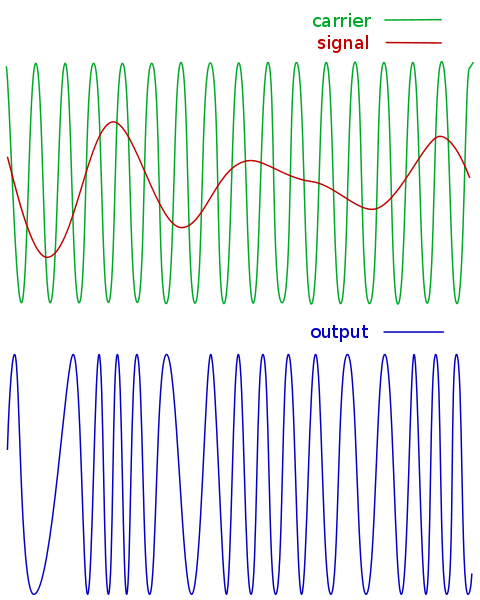
\includegraphics[width=3in]{analog_lab_1_plots/frequency_modulation.png}
\caption{Frequency modulation}\label{fig:frequency_modulation}
\end{figure}

Frequency modulation (FM, see Figure \ref{fig:frequency_modulation}) is a clever scheme for 
encoding a signal.  Amplitude modulation (AM) radio
directly mixes a carrier tone with a signal, so that the amplitude of the signal creates an envelope inside
of which the carrier tone oscillates.  FM instead translates the amplitude of the signal into a change
in the frequency of the carrier tone (see above).  FM radio stations typically transmit between 88 and 108 MHz
in the US.  However, for the purpose of this lab, owing to lack of radio reception in the lab, and the
difficulty in using discrete components at higher frequencies, we will create our own radio station at
1.045 MHz, instead of 104.5 MHz.  Typically, FM radio stations are spaced every 200 kHz, and have a frequency
deviation of $\pm$75 kHz at maximum scale input.

\section{Resistive Voltage Divider}

\subsection{Useful Equations}
\begin{equation}
V=IR
\end{equation}
\begin{equation}
P=IV
\end{equation}

\subsection{Activities}
\begin{itemize}
\begin{figure}[h]
\centering
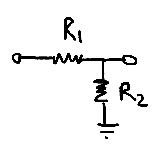
\includegraphics[width=2in]{analog_lab_1_plots/volt_divider.png}
\caption{A voltage divider}\label{fig:volt_divider}
\end{figure}
\item build voltage divider (Figure \ref{fig:volt_divider}) out of two 1k resistors, 
connect input to +5V DC voltage source
\item measure voltage at output
\item measure current (think carefully about where before burning out voltimeter fuse!)
\item apply 1 MHz sine wave, view input and output on oscilloscope
\item append a second voltage divider to the output of the first (choose resistor values carefully)
\item for a voltage divider, is it better to have high impedances or low?  what considerations might
drive you in either direction?
\item from the perspective of the second voltage divider, what is the Th\`evenin equivalent resistance
of the first divider, as seen from its output?
\begin{figure}[ht!]
\centering
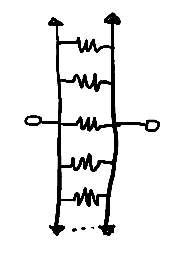
\includegraphics[width=1.5in]{analog_lab_1_plots/resistor_series.png}
\caption{An infinite series of resistors}\label{fig:resistor_series}
\end{figure}
\item if each resistor in Figure \ref{fig:resistor_series} is the same value, what is the equivalent resistance
between the two terminals?  (BTW, I still haven't solved http://xkcd.com/356, but don't get nerd sniped
while doing this lab!)
\end{itemize}

\section{Capacitive Voltage Divider}

\subsection{Useful Equations}
\begin{equation}
I=C\frac{dV}{dt}
\end{equation}

\begin{equation}
Z_C = \frac1{j\omega C}
\end{equation}

\subsection{Activities}

\begin{itemize}
\item build a voltage divider out of two 1$\mu$F capacitors, connect input to 1 MHz sine wave
\item compare input and output on oscilloscope.  is it what you expected? what is the DC level at the output?
resistor?
\item add a 1k resistor to ground at the output, and then for your modified circuit, graph the 
expected $V_{out}/V_{in}$ versus frequency
\end{itemize}

\section{RC filter}

\subsection{Activities}
\begin{itemize}
\item design a high-pass filter with cutoff (-3dB) at 100 kHz
\item design a low-pass filter with the same cutoff
\item plot the expected responses of each.  spot-check with oscilliscope measurements.
\item what could you do to get steeper transitions in RC filters such as these?
\end{itemize}

\section{LC filter}

\subsection{Useful Equations}
\begin{equation}
Z_L = j\omega L
\end{equation}

\begin{equation}
Q = \omega_0 RC = \frac{f_0}{\Delta f_{3dB}}
\end{equation}

\subsection{Activities}
\begin{itemize}
\begin{figure}[h]
\centering
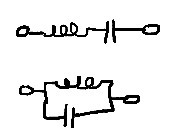
\includegraphics[width=2in]{analog_lab_1_plots/lc_series_parallel.png}
\caption{An inductor in series and in parallel with a capacitor}\label{fig:lc_series_parallel}
\end{figure}
\item plot the theoretical impedance versus frequency of a 1 $\mu$H inductor in parallel 
with and in series with a 1 $\mu$F capacitor (Figure \ref{fig:lc_series_parallel}).
\begin{figure}[h]
\centering
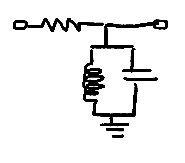
\includegraphics[width=2in]{analog_lab_1_plots/rlc_filter.png}
\caption{A bandpass RLC filter}\label{fig:rlc_filter}
\end{figure}
\item design and build an LC band-pass filter (Figure \ref{fig:rlc_filter}) tuned to 1 MHz
\item choose an R to select a quality factor appropriate for $\Delta f_{3dB}=200 kHz$.
\item for a moment, swap out your C for something quite small (say, 100 pF) and measure empirically
the frequency of peak response.  assuming your inductor value is correct, what is your inferred capacitance?
if this doesn't agree with your C, can you explain why?
\end{itemize}

\section{Diodes}

\begin{itemize}
\item measure the voltage drop over a conducting diode (important: limit current flow with a resistor!)
\item use different resistor values (or a pot) and measure the voltage drop as a function of current
\item use a large ($\pm$ 1V) oscillating signal into the diode and view the original and rectified 
signal on an oscilloscope
\item apply a low-pass filter with time constant of order the input frequency, and view the 
output on an oscilloscope.  generate a plot of what is going on here.
\item suppose you have an oscillating signal whose amplitude is less than the voltage drop across your conducting
diode.  can you come up with a circuit that re-centers your oscillating signal on the threshold 
of diode conduction?
\end{itemize}

\section{FM demodulation}
\begin{figure}[h]
\centering
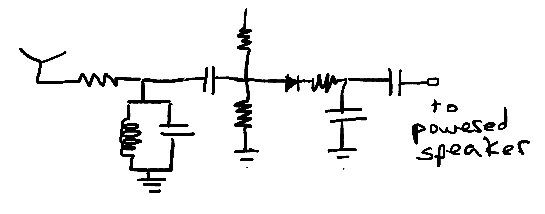
\includegraphics[width=4in]{analog_lab_1_plots/fm_demodulation.png}
\caption{An FM demodulation circuit}\label{fig:fm_demodulation}
\end{figure}

\begin{itemize}
\item use your LC circuit to convert a frequency-modulated signal into an amplitude modulated signal
\item use your diode circuit as an "envelope detector" that filters out the carrier frequency and extracts the
amplitude modulation.  Use a 100 kHz low-pass filter in the envelope detection. (Humans can only hear up to 40 kHz
or so).  You should have something like Figure \ref{fig:fm_demodulation}.
\item connect in our faked FM station at 1.045 MHz
\item connect the output through a coupling capacitor (to remove the DC bias) to amplifying audio speakers
\item enjoy listening to the music
\item fun part: which components of your circuit are strictly necessary?  try removing some of them and see
if it still works?  Draw your circuit as it worked before and after ``contracting'' it.
\item if our station is at 1.045 MHz, why is your LC tuned to 1.0 MHz?  what was relevance of the quality factor?
\end{itemize}

\end{document}
